\chapter{Rancangan}
\label{chap:rancangan}
Bab ini menjelaskan perancangan aplikasi, termasuk algoritma-algoritma untuk mengolah \textit{Google StreetView API}, \textit{Google Directions API}, serta modifikasi yang dilakukan pada aplikasi HelloVR untuk membangun aplikasi \textit{jogging} virtual. 


\section{Rancangan Antarmuka}
Aplikasi yang akan dibangun terdiri atas dua halaman utama, yaitu halaman utama dan halaman VR.

\subsection{Halaman Utama}
\label{subs:main-page}
Halaman utama adalah halaman yang ditampilkan pertama kali saat pengguna membuka aplikasi dengan \textit{portrait layout}. Fungsi halaman ini adalah menerima masukan pengguna, yaitu lokasi asal dan lokasi tujuan saat berlari, serta memicu halaman kedua, yaitu halaman VR. Ada tiga komponen utama dari halaman ini, yaitu dua buah \textit{textbox} dan sebuah tombol. Satu \textit{textbox} adalah \textit{textbox} "\textit{origin}", dan \textit{textbox} yang lain adalah \textit{textbox} "\textit{destination}". Gambar \ref{fig:main-page} menggambarkan tampilan halaman utama.  

\begin{figure}[!hp]
  \centering
    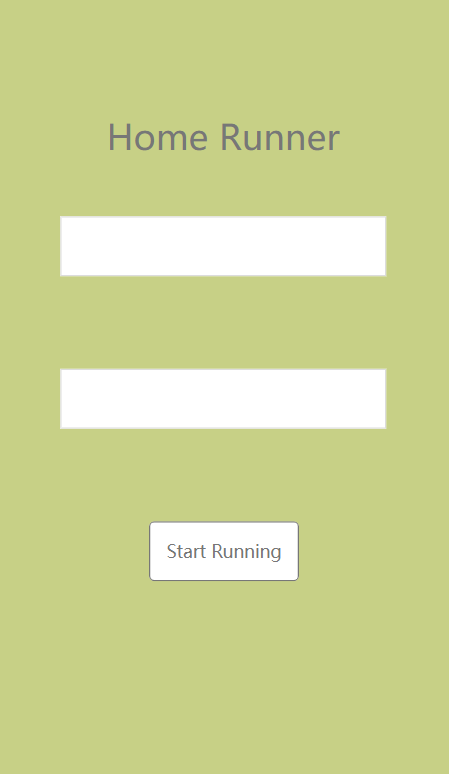
\includegraphics[scale=0.7]{Gambar/mockup-main-activity.png}
    \caption{Rancangan \textit{Activity} utama aplikasi}\label{fig:main-page}
\end{figure}


\subsubsection{\textit{Textbox Origin}} 
\textit{Textbox} adalah komponen pada antarmuka yang menerima masukan pengguna yang berupa tulisan atau \textit{string}. \textit{Textbox} "\textit{origin}" akan menerima masukan pengguna yang merupakan lokasi asal dari rute lari.

\subsubsection{\textit{Textbox Destination}}
\textit{Textbox Destination} adalah \textit{textbox} kedua dan berada di bawah \textit{textbox origin}  akan menerima masukan berupa lokasi tujuan dari rute lari yang dimasukkan pengguna.   

\subsubsection{Tombol ``\textit{Start Running}''}
Tombol "\textit{Start Running}" adalah tombol yang akan memicu halaman VR yang sesuai dengan informasi dari dua \textit{textbox} di atas ketika ditekan. Tombol ini berada di bawah \textit{destination textbox}.

\subsection{Halaman VR}
Halaman VR adalah halaman yang menampilkan pemandangan VR secara VR ketika berlari. Untuk memunculkan halaman ini, pengguna harus menekan tombol dari halaman utama (dijelaskan pada Subbab \ref{subs:main-page}) terlebih dahulu. Karena posisi gawai masih dalam keadaan \textit{portrait}, ada satu halaman terlebih dahulu yang muncul seperti di Gambar \ref{fig:cardboard-page}. 

Halaman ini dimunculkan ketika mengakses \textit{Google Cardboard}. Untuk menuju ke halaman VR, pengguna harus memutar gawai sehingga gawai berada dalam posisi \textit{landscape}. Setelah gawai berada dalam posisi \textit{landscape}, halaman VR akan dimunculkan seperti yang ditunjukkan pada Gambar \ref{fig:vr-page}.

\begin{figure}[h]
	\centering
		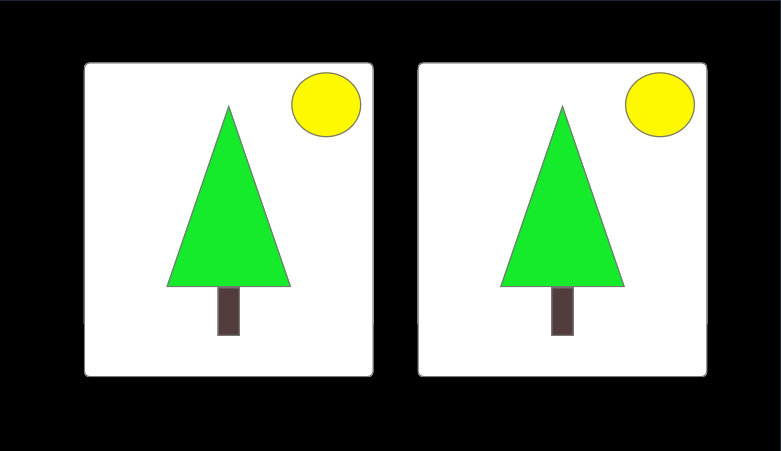
\includegraphics[scale=0.7]{Gambar/mockup-vr-page.png}
	\caption{Rancangan Halaman VR}
	\label{fig:vr-page}
\end{figure}

Pada tampilan VR tersebut, gambar akan berubah-ubah sesuai dengan langkah kaki pengguna. Perubahan tersebut akan terjadi ketika mencapai pengguna mencapai jarak 100 meter. Jika pengguna sudah mencapai tujuan sesuai dengan jarak yang ditempuh, halaman VR akan berhenti mengubah gambar.     

\section{Rancangan Program}
Subbab ini akan menjelaskan rancangan  program, mulai dari rancangan kelas dan algoritma-algoritma yang digunakan pada \textit{method-method} yang penting. 

\subsection{Rancangan Kelas}
Rancangan kelas dari aplikasi akan menggunakan seluruh bagian pada aplikasi HelloVR dan beberapa tambahan kelas. Gambar \ref{fig:class-diagram} menunjukkan atribut-atribut dan \textit{method-method} dari masing-masing kelas, serta hubungan antara satu kelas dan kelas-kelas lain. 

\begin{figure}[h]
	\centering
		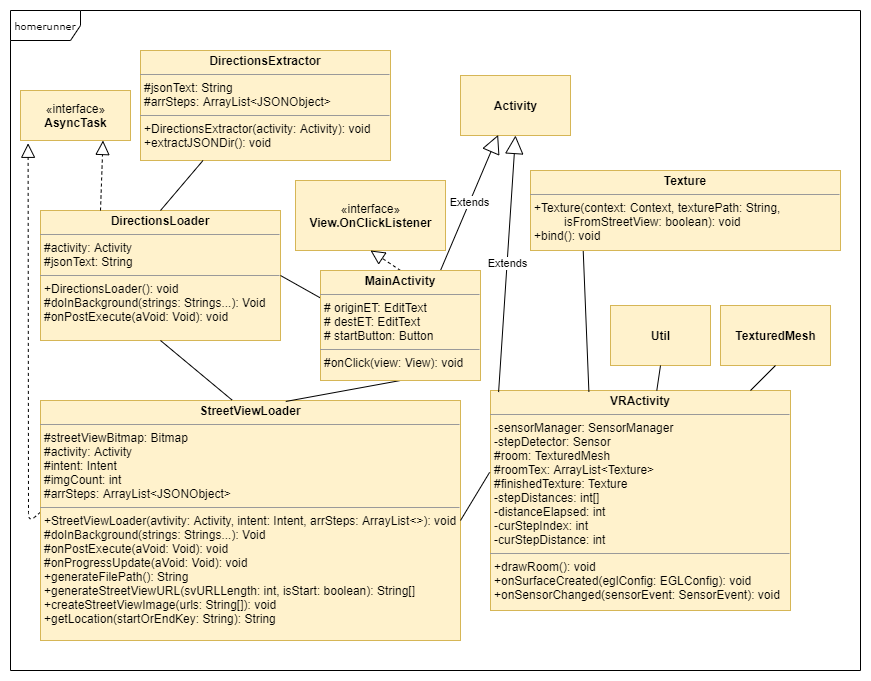
\includegraphics[scale=0.6]{Gambar/class-diagram.png}
	\caption{Diagram \textit{class} dari Aplikasi}
	\label{fig:class-diagram}
\end{figure}

Beberapa kelas di Gambar \ref{fig:class-diagram} tidak memiliki deskripsi lebih karena berasal dari \textit{library} Java ataupun \textit{Google VR SDK}. Kelas-kelas yang ditambahkan adalah:

%Lengkapi penjelasan
\begin{enumerate}
	\item \texttt{MainActivity}
	
	Kelas yang mengelola halaman utama. Atribut yang dimiliki kelas ini:
	
	\begin{itemize}
		\item \texttt{protected EditText originET}
		
		Bagian dari antarmuka yang dapat menerima masukan lokasi asal dari rute lari.
		\item \texttt{protected EditText destET}
		
		Bagian antarmuka yang dapat menerima masukan lokasi tujuan dari rute lari.
		\item \texttt{protected Button startButton}
		
		Tombol yang digunakan untuk memicu halaman VR.
		\item \texttt{protected StreetViewLoader streetViewLoader}
		
		Atribut dari \textit{loader} gambar \textit{StreetView} untuk menginisialisasi di halaman VR.
	\end{itemize}
	
	\textit{Method-method} yang dimiliki kelas ini adalah:
	
	\begin{itemize}
		\item \texttt{protected void onClick(View view)}
		
		\textit{Method} yang dijalankan ketika komponen yang sudah dipasangkan \texttt{onClickListener} ditekan. 
		\item \texttt{public String[] generateStreetView(int svUrlLength)}
		
		\textit{Method} ini akan men-\textit{generate} gambar \textit{StreetView} dari sekeliling pemandangan. 
		
		Parameter:
		
		\begin{itemize}
			\item \texttt{int svUrlLength}
			
			Parameter ini menyatakan berapa banyak \textit{string} URL untuk mendapatkan gambar-gambar StreetView.
		\end{itemize}
		
	\end{itemize}
	\item \texttt{HelloVRActivity}
	
	\textit{Class} yang mengelola halaman VR. Atribut-atribut yang dimiliki \textit{class} ini adalah:
	
	\begin{itemize}
		\item \texttt{private SensorManager sensorManager}
		
		Atribut yang mengatur sensor dari gawai Android.
		\item \texttt{private Sensor stepDetector}
		
		Sensor pendeteksi langkah kaki. 
		\item \texttt{private StreetViewLoader sVLoader}
		
		Pemuat gambar StreetView.
		\item \texttt{private ArrayList arrSteps}
		
		\textit{ArrayList} dari semua \textit{step-step} dari rute lari.
		\item \texttt{private int distanceElapsed}
		
		Atribut ini menyimpan jarak yang sudah ditempuh pengguna.
		\item \texttt{private int curStepIndex}
		
		Atribut yang menyimpan \textit{index} dari \textit{step} yang sedang ditempuh saat ini.
		\item \texttt{private int curStepDistance}

		Atribut yang menyimpan jarak dari \textit{step} saat ini.		
	\end{itemize}
	
	\textit{Method-method} yang dimiliki \textit{class} ini adalah:
	
		\begin{itemize}
			\item \texttt{public void drawRoom()}
			
			\textit{Method} untuk menggambar ruangan tiga dimensi.
			\item \texttt{public void onSurfaceCreated(EFLConfig eflConfig)}
			
			\textit{Method} yang dipanggil ketika permukaan VR diciptakan. Parameter yang dimiliki \textit{method} ini adalah:
			
			\begin{itemize}
				\item \texttt{EGLConfig eglConfig}
				
			Konfigurasi dari  \textit{OpenGL renderer}. 				
			\end{itemize}
			
		\item \texttt{public void loadJSONDir()}
				
				\textit{Method} untuk  memuat \textit{file} JSON dari \textit{Google Directions}.
		\end{itemize}
	
	\item \texttt{StreetViewLoader}
	
	\textit{Class} yang berfungsi untuk memuat gambar \textit{StreetView} dan menyatukan semua gambar itu, membentuk gambar pemandangan yang utuh. Atribut-atribut yang dimiliki \textit{class} ini adalah:
	
	\begin{itemize}
		\item \texttt{protected MainActivity mainActivity}
		\textit{Activity} yang dihubungkan dengan \textit{class} ini  sehingga komunikasi antara objek dua kelas ini dapat terjadi. 		
		
		\item \texttt{protected String filepath}
		
		Atribut yang menyimpan \textit{filepath} untuk menyimpan \textit{file} dari gambar \textit{StreetView} yang sudah selesai diolah.
		\item \texttt{protected Bitmap streetViewBitmap}
		
		Atribut untuk menyimpan \textit{bitmap} dari gambar \textit{StreetView}.
		\item \texttt{protected Activity activity}
		
		Atribut dari \textit{activity} yang memanggil \textit{method} dari \textit{class} ini sehingga data dan nilai yang sudah diperoleh dari \textit{class} ini dapat diserahkan pada \textit{activity} ini.
		\item \texttt{protected Intent intent}  
		
		\textit{Intent} dari \textit{activity} yang memicu \textit{class} ini untuk bekerja.
	\end{itemize}
	
	\textit{Method-method} yang dimiliki \textit{class} ini adalah:
	
	\begin{itemize}
		\item \texttt{protected doInBackground(Strings... strings}
		
		\textit{Method} yang memuat dan menyatukan gambar-gambar \textit{StreetView API}, yang dijalankan pada \texttt{AsyncTask} berbeda. Parameter yang dimiliki \textit{method} ini adalah:
		
		\begin{itemize}
			\item \texttt{Strings.. strings}
			
			Kumpulan \textit{string} dari URL-URL untuk memanggil \textit{StreetView API} dari \textit{heading} yang berbeda-beda.
		\end{itemize}				
		 
		\item \texttt{protected Void onPostExecute(Void aVoid)}
		
		\textit{Method} yang dipanggil setelah \texttt{doInBackground()} selesai dijalankan.
		\item \texttt{private void cleanUpMainActivity()}
		
		\textit{Method} yang dijalankan di \textit{method} \texttt{onPostExecute()} ketika \textit{class} ini dipicu dari \textit{activity} yang merupakan \textit{instance} dari \texttt{MainActivity}.
		\item \texttt{private void cleanUpVrActivity()}
		
		\textit{Method} yang dijalankan di \textit{method} \texttt{onPostExecute()} ketika \textit{class} ini dipicu dari \textit{activity} yang merupakan \textit{instance} dari \texttt{HelloVrActivity}.
		
		\textit{Method} yang dijalankan ketika 
	\end{itemize}
	
	\item \texttt{DirectionsLoader}
	
	\textit{Class} yang memuat JSON dari rute lari. Atribut-atribut yang dimiliki kelas ini adalah:
	\begin{itemize}
		\item \texttt{protected String jsonText}
		
		Atribut yang menyimpan \textit{text} yang diperoleh dari \textit{Directions API}.
	\end{itemize}
	
	\textit{Method-method} yang dimiliki \textit{class} ini adalah:
	
	\begin{itemize}
		\item \texttt{public DirectionsLoader()}
		
		\textit{Constructor} dari \textit{DirectionsLoader()}	
		\item \texttt{protected Void doInBackground(Strings... strings)}
		
		\textit{Method} yang dijalankan di \texttt{AsyncTask} berbeda, yaitu untuk memuat \textit{file} JSON \textit{Directions API}.
		\item \texttt{protected Void onPostExecute(Void aVoid)}
		
		\textit{Method} yang dijalankan setelah \textit{method} \texttt{doInBackgroud()} selesai dijalankan, untuk memproses \textit{text} dari \textit{Directions API}. 
	\end{itemize} 
\end{enumerate} 


\subsection{Algoritma-Algoritma yang digunakan}
Ada beberapa algoritma yang digunakan   untuk melakukan beberapa proses seperti mengolah \textit{Google StreetView API},\textit{Google Directions API}, dan menampilkan .

\subsubsection{Algoritma Memperoleh dan Mengolah \textit{Google StreetView API}} 
\textit{StreetView API} berfungsi untuk memuat gambar pemandangan dan menggunakan menggunakan HTTP/HTTPS. Karena sekali pemanggilan hanya menghasilkan gambar dari satu arah pemandangan, empat gambar dari empat pandangan haruslah diunduh terlebih dahulu. Setelah semua gambar itu terunduh, semua gambar itu disatukan, menjadi satu gambar untuk menjadi tekstur bangun ruang silinder. Algoritma yang digunakan untuk menyatukan gambar-gambar tersebut. Setelah gambar-gambar itu sudah disatukan, gambar tersebut harus disimpan di dalam \textit{file} pada \textit{StreetView} tersebut adalah: Langkah-langkah untuk memuat dan mengolah gambar-gambar untuk menyajikan gambar pemandangan yang utaha adalah:

	\begin{enumerate}
		\item Memuat gambar \textit{StreetView} dari semua arah lewat HTTP/HTTPS. 
		
		\item Menggabungkan gambar  \textit{StreetView} dari semua arah yang sudah dimuat.
		
		\item Menyimpan gambar dalam \textit{cache}.
	\end{enumerate}	
	
\begin{figure}[h]
	\centering
		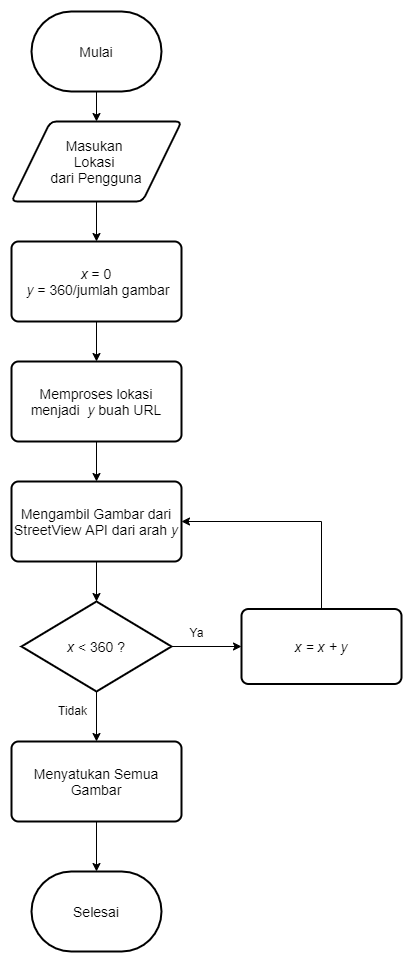
\includegraphics[scale=0.6]{Gambar/streetview-flowchart.png}
	\caption{\textit{Flowchart} dari Proses Memperoleh dan Menyatukan Gambar dari \textit{StreetView API}}
	\label{fig:streetview-flowchart}
\end{figure}

Gambar \ref{fig:streetview-flowchart} menggambarkan proses-proses pemanggilan StreetView API. Peubah \textit{x} pada \textit{flowchart} menunjuk pada nilai \textit{heading} dari gambar yang akan diperoleh, sedangkan peubah \textit{y} merupakan selisih derajat dari satu gambar ke gambar yang lain. Nilai 360 menunjuk pada 360 derajat dalam satu putaran. Untuk mendapatkan pemandangan yang sekeliling yang penuh, gambar dari setiap derajat ke-\textit{x} selama nilai \textit{x} masih bernilai lebih kecil dari 360. Setelah gambar-gambar  itu sudah diperoleh dari \textit{StreetView API}, gambar-gambar tersebut harus disatukan, barulah gambar itu bisa digunakan sesuai kebutuhan.


\subsubsection{Pemanfaatan \textit{Google Directions API}}
\textit{Directions API} adalah \textit{API} yang menggunakan protokol HTTP/HTTPS dan menghasilkan keluaran dalam bentuk JSON. Untuk memuat JSON berisi rute perjalanan dari asal sampai tujuan, pemanggilan \textit{Directions API} harus dilakukan melalui HTTP/HTTPS.

\begin{algorithm}
	\caption{Algoritma Mengunduh JSON dari \textit{Directions API} dan \textit{Parsing}}
	\label{alg:algoritma-directions-parsing}
	\begin{algorithmic}[1]
	\Function{processJSONDirections}{$originLoc$,$destLoc$}
		\State $dirText \gets getJSONFromDirAPI(originLoc,destLoc)$ 
		
		\State $dirJSON \gets toJSON(dirText)$	
		
		\State $jsonRoute \gets dirJSON.getJSONObject("routes")$
		
		\State $jsonArrLegs \gets jsonRoute.getJSONArray("legs")$

		\State Declare Array$processedJSONObj$		
		
		\For $ elements in jsonArrLegs$
		\State $jsonLegs \gets element.getJSONObject("legs") $

		\State $jsonArrSteps \gets jsonLegs.getJSONArray("steps")$		
		
		\State Insert all elements from $jsonArrSteps$ to $processedJSONObject$ 
			
		
		\EndFor
%		\State $lastT \gets currT$
%		
%		\If {hill and valley time values has been set \textbf{AND} all condition have been met}
%			\Return $true$
%		\Else {
%			\Return $false$}
%		\EndIf
	\EndFunction  
	\end{algorithmic}
\end{algorithm}

Setelah JSON rute diperoleh, JSON rute lari dapat digunakan dengan membaca atribut dan nilai-nilainya sesuai kebutuhan. Beberapa nilai atribut dalam JSON ini  berupa JSON \textit{object}, ada yang berupa JSON \textit{array}. Karena hal ini,  \textit{parsing} dari JSON ini harus dilakukan sesuai dengan ketentuan tersebut. Algoritma \textit{parsing} dari JSON \textit{Directions} dipaparkan pada \ref{alg:algoritma-directions-parsing}. 

Setelah JSON dari \textit{Directions API} diunduh, \textit{parsing} adalah langkah selanjutnya untuk mengambil informasi yang dibutuhkan. Karena bagian \textit{steps} yang harus diambil, 

\subsubsection{Pemanfaatan Sensor \textit{Step Detector}}
Sensor \textit{step detector} digunakan untuk mendeteksi langkah kaki pengguna. Untuk membentuk skenario yang tepat untuk memungkinkan perubahan pemandangan yang sudah ditangani oleh \textit{StreetView} dan \textit{Directions API}, waktu perubahan dari pemandangan itulah yang harus ditangani. Sensor \textit{step detectorlah} yang akan menangani bagian waktu perubahan pemandangan. 

Sebuah peubah bertipe numerik (\textit{integer}) yang menandakan \textit{progress} perjalanan pelari, lalu harus ada sebuah konstan yang menyatakan jarak dari satu langkah. Saat sensor \textit{step detector} mendeteksi adalah sebuah langkah kaki, peubah dari \textit{progress} akan ditambahkan dengan nilai konstan jarak satu langkah kaki. Jika nilai peubah \textit{progress} sudah sampai  jarak tertentu, pemandangan akan berubah, sesuai dengan \textit{Directions API}. 

%\section{\textit{Folder Assets}}
%
%\textit{Folder assets} mengandung \textit{asset-asset} multimedia seperti gambar dan \textit{audio}. 
%Menghapus \textit{file-file} dari aplikasi HelloVR. 
%
%Mengganti CubeRoom.obj dengan file OBJ dengan bangun ruang silinder.
%
%Mengganti file CubeRoom\_BakedDiffuse.png, menggantinya dengan gambar \textit{StreetView} yang sudah disatukan. 
